\documentclass{article}
\usepackage[utf8]{inputenc}
\usepackage[]{graphicx}
\usepackage{float}
\usepackage{amsthm}
\usepackage[colorlinks=true, allcolors=blue]{hyperref}

\newtheorem{algorithm}{Algorithm}

\begin{document}
\title{RODM}
\author{Aamr \textsc{El Kazdadi}\\
        El Mahdi \textsc{Chayti}}
\date{}
\maketitle
\section*{Practical 1}%
\subsection*{Exercise 2}%
\label{sub:tp1ex2}
The size of the graph is calculated by iterating over the text file and
counting the number of lines containing pairs of integers.
Note that this is to be used on raw graphs, as cleaned ones already contain the
number of nodes and edges on the first line.
As a result of this and the fact that we avoid storing the edges in memory, the
program doesn't account for potential duplicates.

\subsection*{Exercise 3}%
\label{sub:tp1ex3}
The program first counts the number of lines using ``wc -l", to tell how much
memory it should allocate for the edge list, then we iterate over each line
and add the edges to the list in the correct order.
(tail is strictly smaller than head)\\
We then sort the edge list in lexicographical order.
(the order is based on tail of edge, and in case of equality, on the head of the
edge)\\
We iterate over the edge list to count the number of non duplicate edges,
and write the number of nodes and number of edges to a new text file.\\
We iterate once again on the list of edges and save them to a new text file,
skipping over duplicates. Note that node indices are shifted so that they start
from 0.

\subsection*{Exercise 4}%
\label{sub:tp1ex4}
We read the number of nodes and the number of edges from the cleaned files, and
allocate memory for a list of node degrees.\\
We iterate over the (cleaned) file of list of edges, and for each edge, we
increment the degrees of its tail and its head.

\subsection*{Exercise 5}%
\label{sub:tp1ex5}
We read the number of nodes and the number of edges from the cleaned files, and
allocate memory for a list of edges and a list of node degrees.\\
We first calculate the degrees of nodes.\\
Then we iterate over the edge list and calculate the desired quantity.
\begin{table}[!ht]
    \centering
    \label{tab:label}
    \begin{tabular}{lrrr}
        Graph & $Q_G$ & degree computation& $Q_G$ computation\\
        Email&
        103747042&
        0.001894s&
        0.000026s\\
        Amazon&
        103415531&
        0.136159s&
        0.003211s\\
        Live Journal&
        789000450609&
        5.016865s&
        0.126856s\\
        Orkut&
        22292678512329&
        17.231983s&
        0.430236s\\
        Friendster&
        379856554324947&
        389.599227s&
        24.310711s\\
    \end{tabular}
\end{table}

\subsection*{Exercise 6}%
\label{sub:tp1ex6}
We compute the degree list and save it to a file, we then count the number of
occurences of each value and plot the distribution.

\begin{figure}[H]
    \centering
    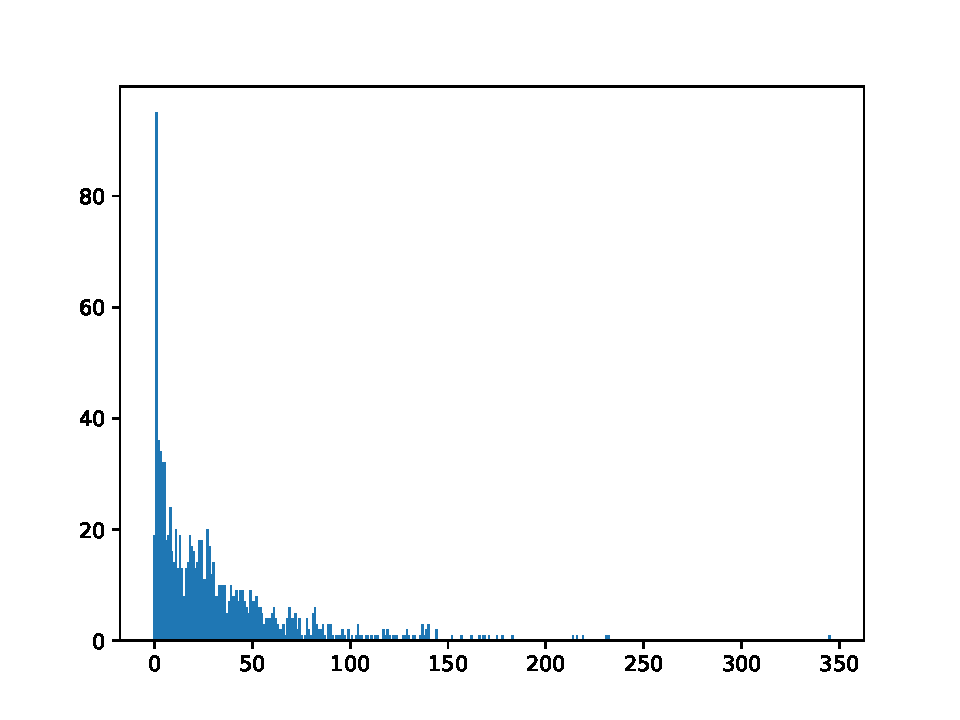
\includegraphics[width=0.8\textwidth]{plots/email-Eu-core.pdf}
    \caption{Email graph degree distribution}
    \label{fig:email-deg}
\end{figure}

\begin{figure}[H]
    \centering
    \includegraphics[width=0.8\textwidth]{plots/{com-amazon.ungraph}.pdf}
    \caption{Amazon graph degree distribution}
    \label{fig:amazon-deg}
\end{figure}

\begin{figure}[H]
    \centering
    \includegraphics[width=0.8\textwidth]{plots/{com-lj.ungraph}.pdf}
    \caption{Live Journal graph degree distribution}
    \label{fig:lj-deg}
\end{figure}

\begin{figure}[H]
    \centering
    \includegraphics[width=0.8\textwidth]{plots/{com-orkut.ungraph}.pdf}
    \caption{Orkut graph degree distribution}
    \label{fig:orkut-deg}
\end{figure}

\begin{figure}[H]
    \centering
    \includegraphics[width=0.8\textwidth]{plots/{com-friendster.ungraph}.pdf}
    \caption{Friendster graph degree distribution}
    \label{fig:friend-deg}
\end{figure}

\subsection*{Exercise 7}%
\label{sub:tp1ex7}
The list of edges is stored ``as is".\\
The adjacency matrix is represented as an array of arrays of char values.
Each array contains a row of the matrix, and each char value contains 8
consecutive elements of the row.\\
Degrees of nodes are first calculated, then the adjacency array is stored as
specified in the course.

\subsection*{Exercise 8}%
\label{sub:tp1ex8}
We allocate an array to contain the component index of each node, initialized
to -1, and we set the count of components to 0.\\
We iterate over the nodes, and whenever a component of -1 is found, we set its
compoenent index as well as the ones of all the nodes connected to it (found by
a breadth-first search) to the current count.
We then increment the compoenent count by 1.

\begin{table}[htpb]
    \centering
    \begin{tabular}{lrr}
        Graph & \% nodes in largest component & Diameter lower bound\\
        Email&
        98.109453\%&
        7\\
        Amazon&
        61.045008\%&
        47\\
        Live Journal&
        99.044330\%&
        21\\
        Orkut&
        99.993979\%&
        10\\
        Friendster&
        52.555613\%&
        37\\
    \end{tabular}
\end{table}

\section*{Practical 2}%
\label{sec:tp2}
\subsection*{Exercise 1}%
\label{sub:tp2ex1}
We read the directed edge list and store it as an adjacency array.
The matrix vector product and the PageRank algorithm are implemented as
specified in the course.\\
For $\alpha = 0.15$, the algorithm converges in 16 iterations.\\
Top 5 pages
\begin{itemize}
    \item United States
    \item United Kingdom
    \item Germany
    \item 2007
    \item 2006
\end{itemize}
Bottom 5 pages
\begin{itemize}
    \item WCXL
    \item WGCC-FM
    \item WAFJ
    \item WBFR
    \item Leroy Township, Michigan
\end{itemize}

\subsection*{Exercise 2}%
\label{sub:tp2ex2}
We use linear scales for degrees and log scales for pagerank values, since they
take values close to 0 with different orders of magnitude.\\
PageRank is positively correlated with the in-degree\\
PageRank is slightly negatively correlated with the out-degree\\
The PageRank values are positively correlated.

\begin{figure}[H]
    \centering
    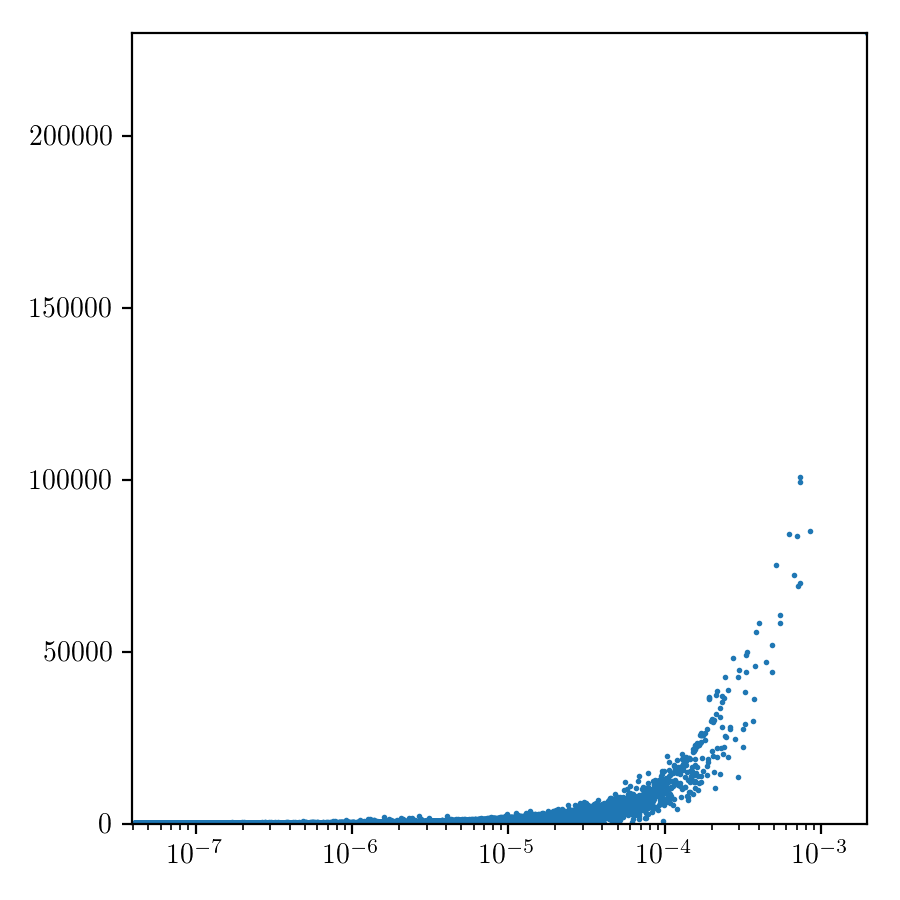
\includegraphics[width=0.65\textwidth]{plots/1.png}
    \caption{$x =$ PageRank with $\alpha = 0.15$, $y = $ in-degree}
    \label{fig:1}
\end{figure}

\begin{figure}[H]
    \centering
    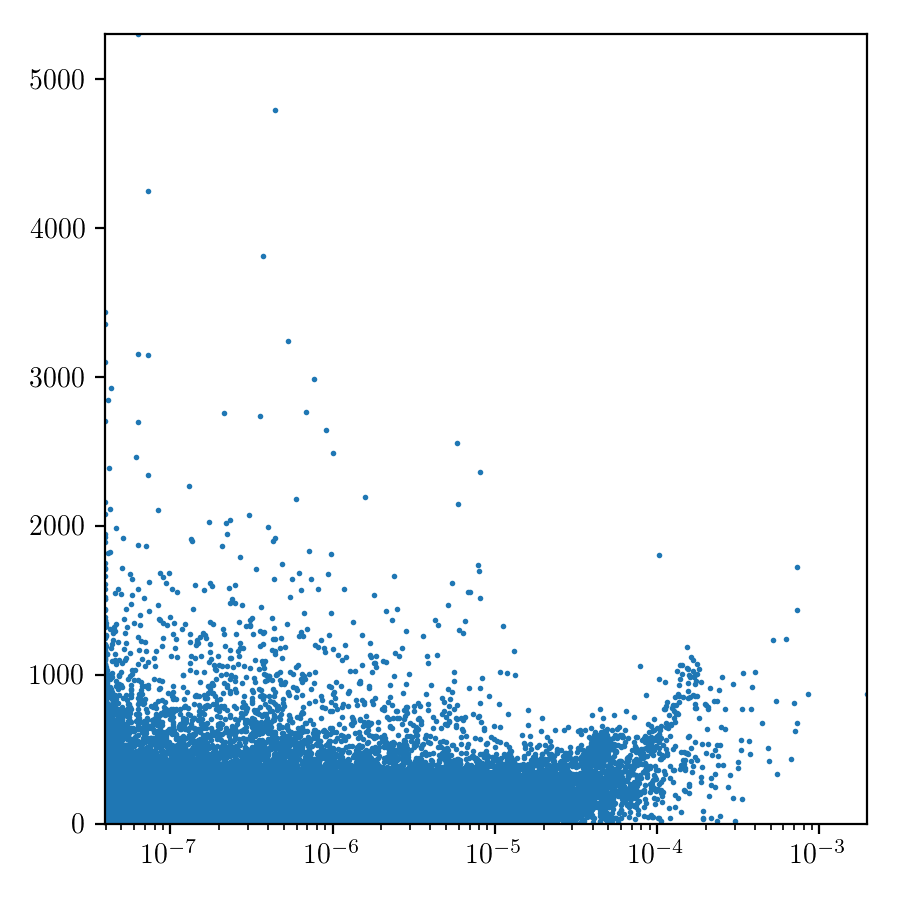
\includegraphics[width=0.65\textwidth]{plots/2.png}
    \caption{$x =$ PageRank with $\alpha = 0.15$, $y = $ out-degree}
    \label{fig:2}
\end{figure}

\begin{figure}[H]
    \centering
    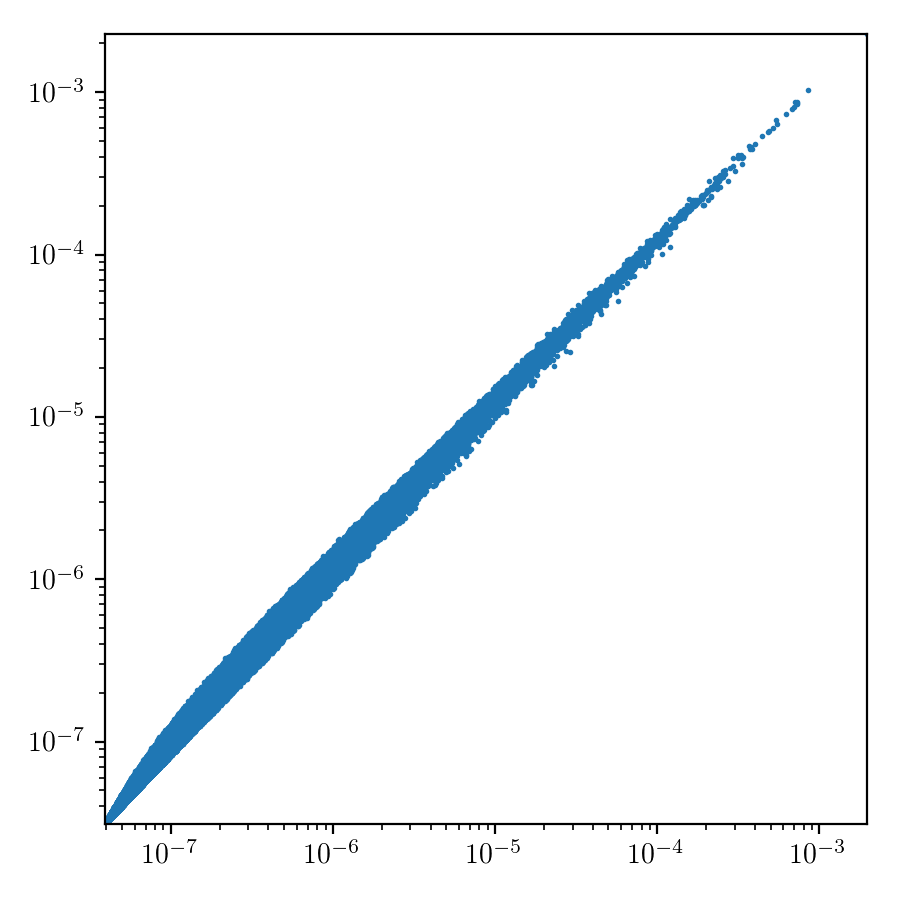
\includegraphics[width=0.65\textwidth]{plots/3.png}
    \caption{$x =$ PageRank with $\alpha = 0.15$, $y = $ PageRank with $\alpha = 0.1$}
    \label{fig:3}
\end{figure}

\begin{figure}[H]
    \centering
    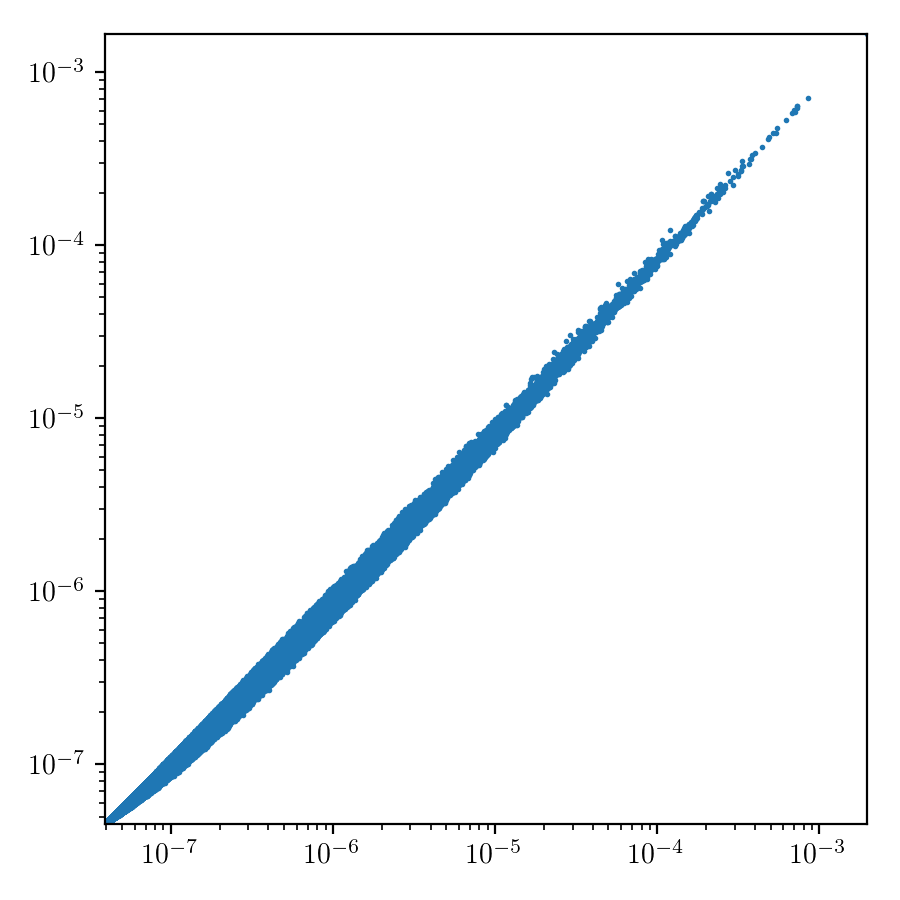
\includegraphics[width=0.65\textwidth]{plots/4.png}
    \caption{$x =$ PageRank with $\alpha = 0.15$, $y = $ PageRank with $\alpha = 0.2$}
    \label{fig:4}
\end{figure}

\begin{figure}[H]
    \centering
    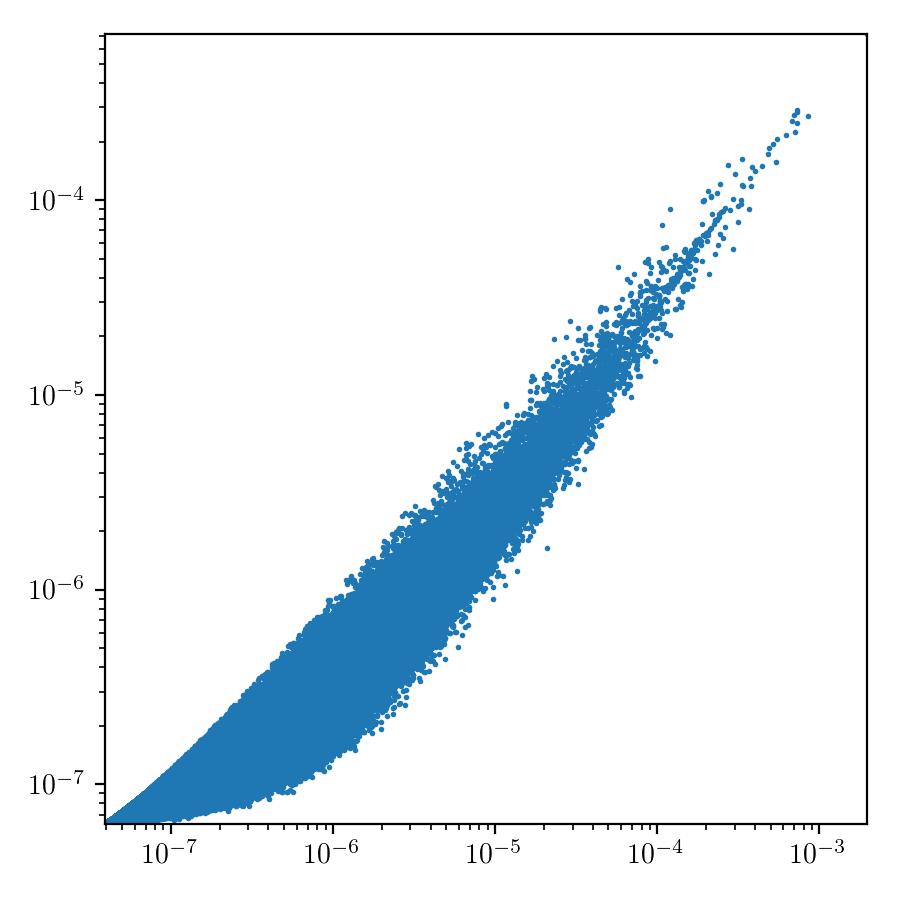
\includegraphics[width=0.65\textwidth]{plots/5.png}
    \caption{$x =$ PageRank with $\alpha = 0.15$, $y = $ PageRank with $\alpha = 0.5$}
    \label{fig:5}
\end{figure}

\begin{figure}[H]
    \centering
    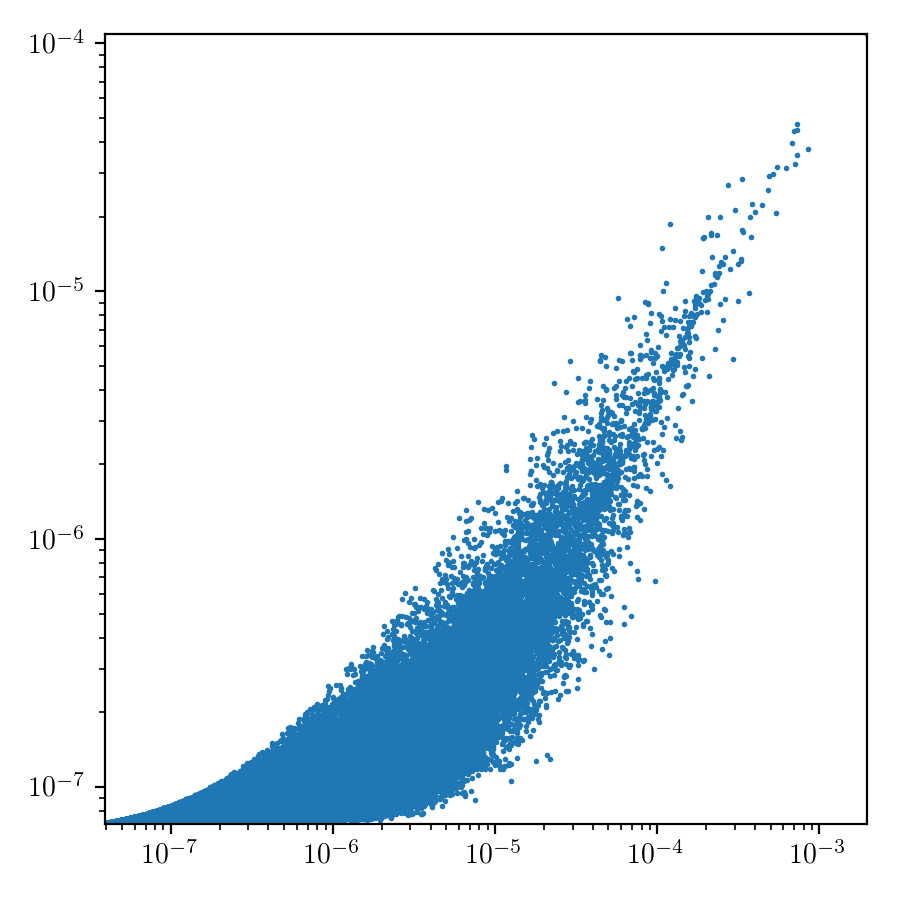
\includegraphics[width=0.65\textwidth]{plots/6.png}
    \caption{$x =$ PageRank with $\alpha = 0.15$, $y = $ PageRank with $\alpha = 0.9$}
    \label{fig:6}
\end{figure}

\subsection*{Exercise 3}%
\label{sub:tp2ex3}
\begin{table}[!ht]
    \centering
    \begin{tabular}{lrr}
        Graph & Running time & Core value\\
        Email&
        0.000548s&
        34\\
        Amazon&
        0.167125s&
        6\\
        Live Journal&
        4.625723s&
        360\\
        Orkut&
        16.438648s&
        253
    \end{tabular}
\end{table}

\section*{Practical 3}%
\label{sec:tp3}
\subsection*{Exercise 1}

\begin{figure}[!ht]
\centering
\begin{minipage}{.33\textwidth}
  \centering
  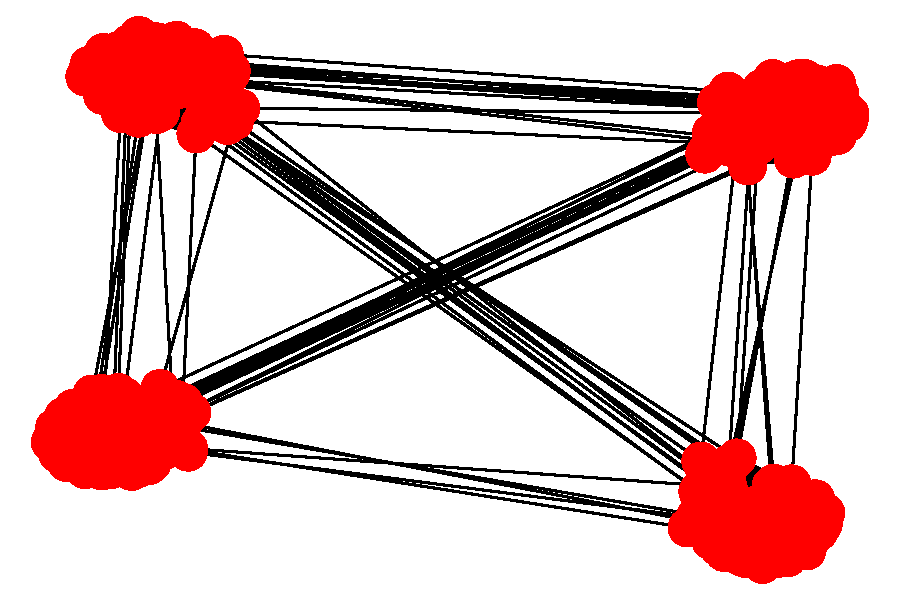
\includegraphics[width=\linewidth]{plots/graph1p=0,9q=0,001.pdf}
  \caption{p=0.9 q=0.001}
\end{minipage}%
\begin{minipage}{.33\textwidth}
  \centering
  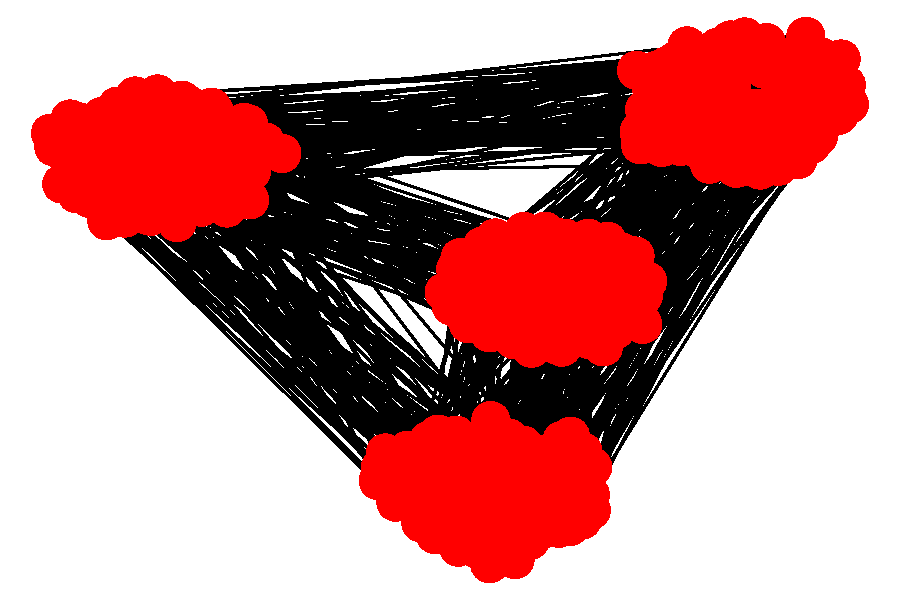
\includegraphics[width=\linewidth]{plots/graph2p=0,8q=0,01.pdf}
  \caption{p=0.8 q=0.01}
\end{minipage}
\begin{minipage}{.33\textwidth}
  \centering
  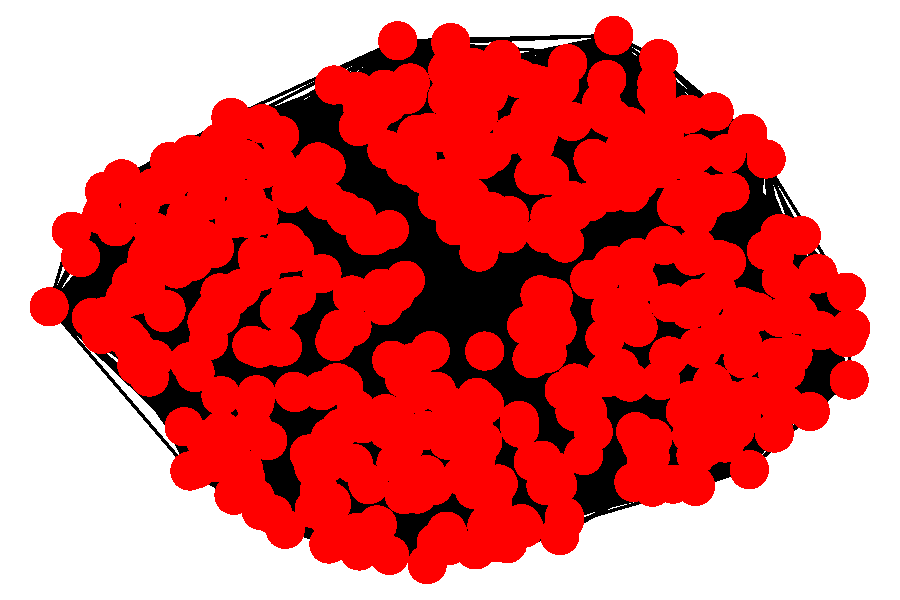
\includegraphics[width=\linewidth]{plots/graph3p=0,8q=0,02.pdf}
  \caption{p=0.8 q=0,02}
\end{minipage}
\end{figure}

Increasing $ \frac{p}{q} $ makes the community structure more evident.
And in the limit case of $ \frac{p}{q} \to 1 $, the communities become
indistinguishable.

\subsection*{Exercise 2}
The label propagation algorithm is implemented as specified in the course.
We apply the Label propagation algorithm to the first graph to the right, the
result is in figure \ref{fig:LP}.

\begin{figure}[!ht]
    \centering
    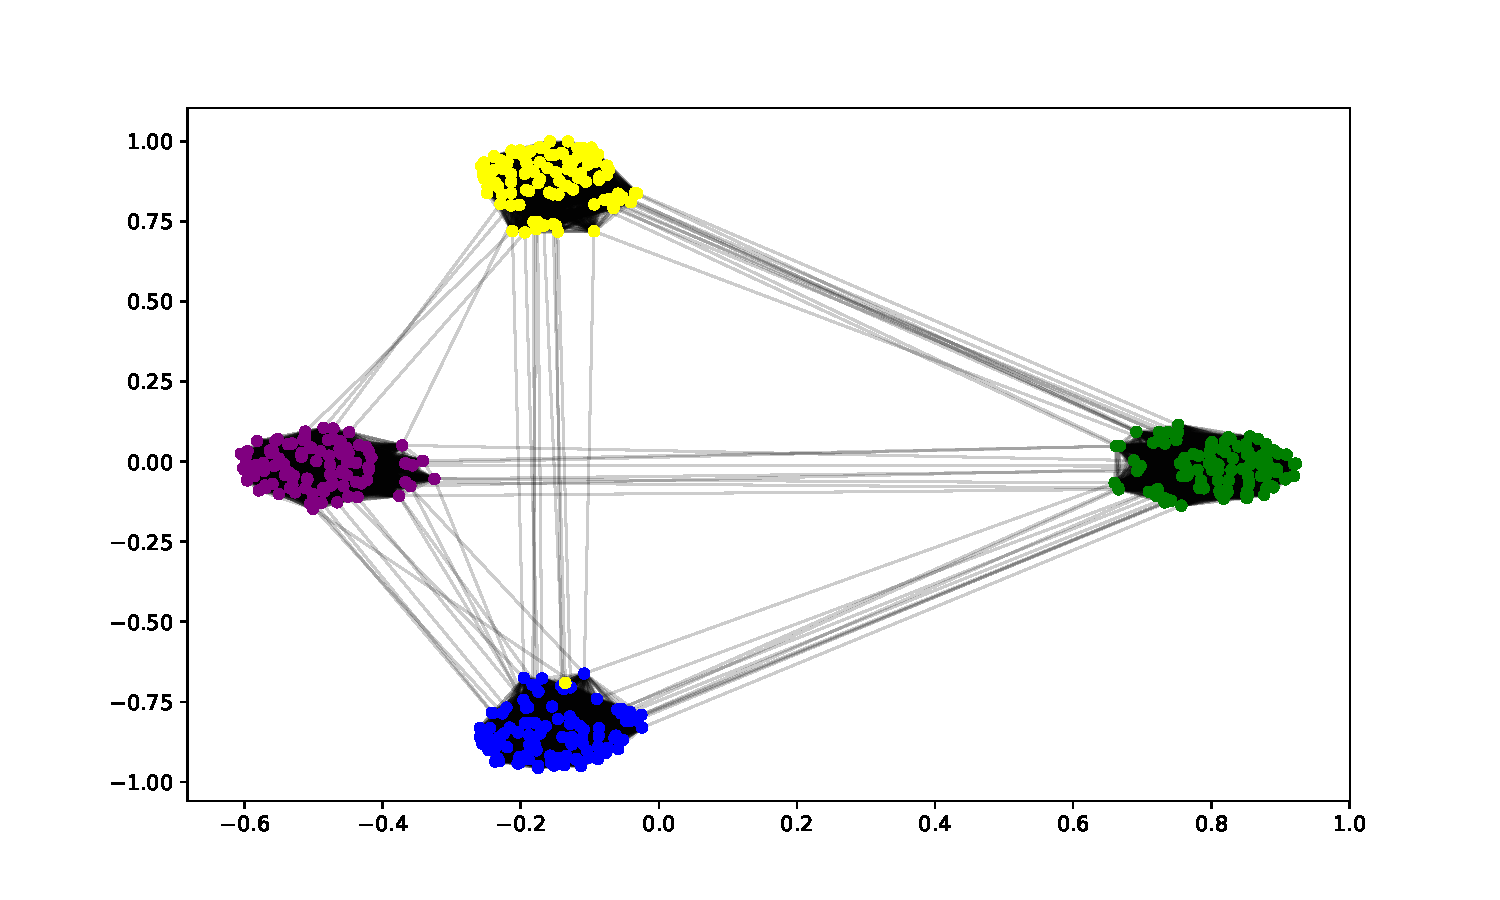
\includegraphics[width=\linewidth]{plots/images1/LabelPropagation.pdf}
    \caption{Label propagation}
    \label{fig:LP}
\end{figure}

We see that it did get it almost right(except for one node).\\
It took $\approx 0.015$ seconds to classify the four communities on this graph of 400 nodes.

\subsection*{Exercise 3}
\begin{algorithm}
Until there is no change in the communities, we shuffle the nodes, and for each
node, we look for its neighbour that has the minimal degree (we may also look
only among the neighbours that verify a criterion like number of neighbours
greater than a threshold) and enforce that they be in the same community, we do
so until there is no change in the communities.
\end{algorithm}

The intuition behind is that the nodes who have connections outside their
community tend to have a greater degree than those with connections limited to
their own community.
This tends to work well on graphs with clear community structure.

We were inspired by an algorithm called minimal degree that consists in
maximizing the minimal degree in a community(using local search for example),
but as it is not evident to optimize such algorithm (need for intelligent local
updates of some numbers that characterize the community) we used a version that
mix label propagation and this algorithm.

The result we get when applying this algorithm to the first graph is on figure \ref{fig:mindeg}.

\begin{figure}[!ht]
    \centering
    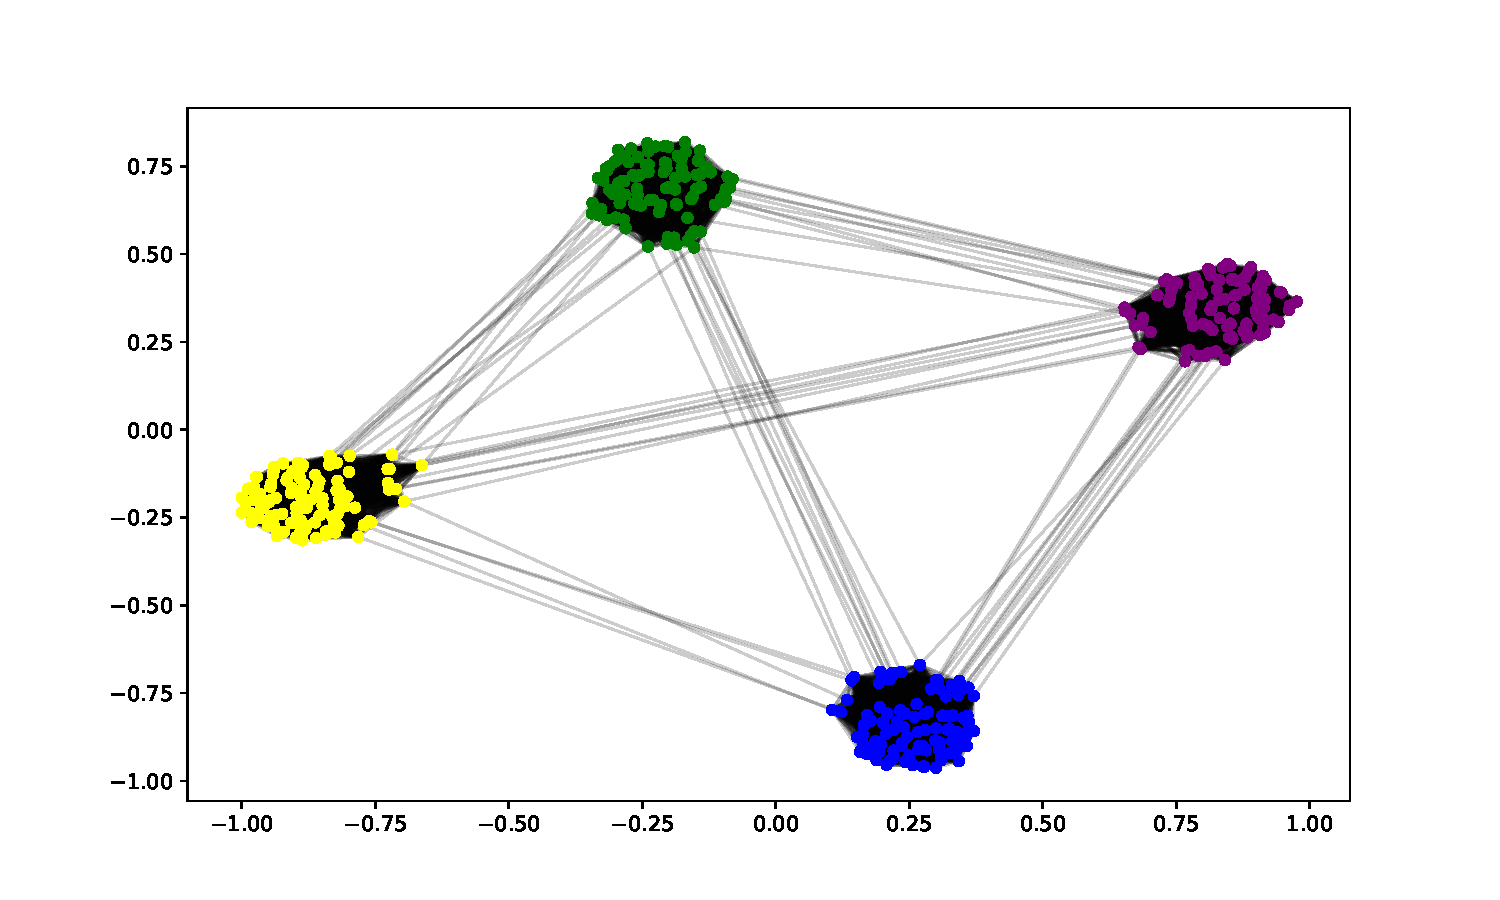
\includegraphics[width=\linewidth]{plots/images1/ex3minimalDegree.pdf}
    \caption{minimal degree algorithm}
    \label{fig:mindeg}
\end{figure}

The algorithm performed a perfect community detection here and did better than
the Label Propagation.\\
It took $\approx 0.018$ seconds (needs slightly more time compared to Label
Propagation) to classify the four communities on this graph of 400 nodes.

\subsection*{Exercise 4}

We used the Louvain algorithm%
\footnote{\url{https://python-louvain.readthedocs.io/en/latest/}}
and applied it to the first graph, the result is shown in figure
\ref{fig:louv}.
\newpage
\begin{figure}[!ht]
    \centering
    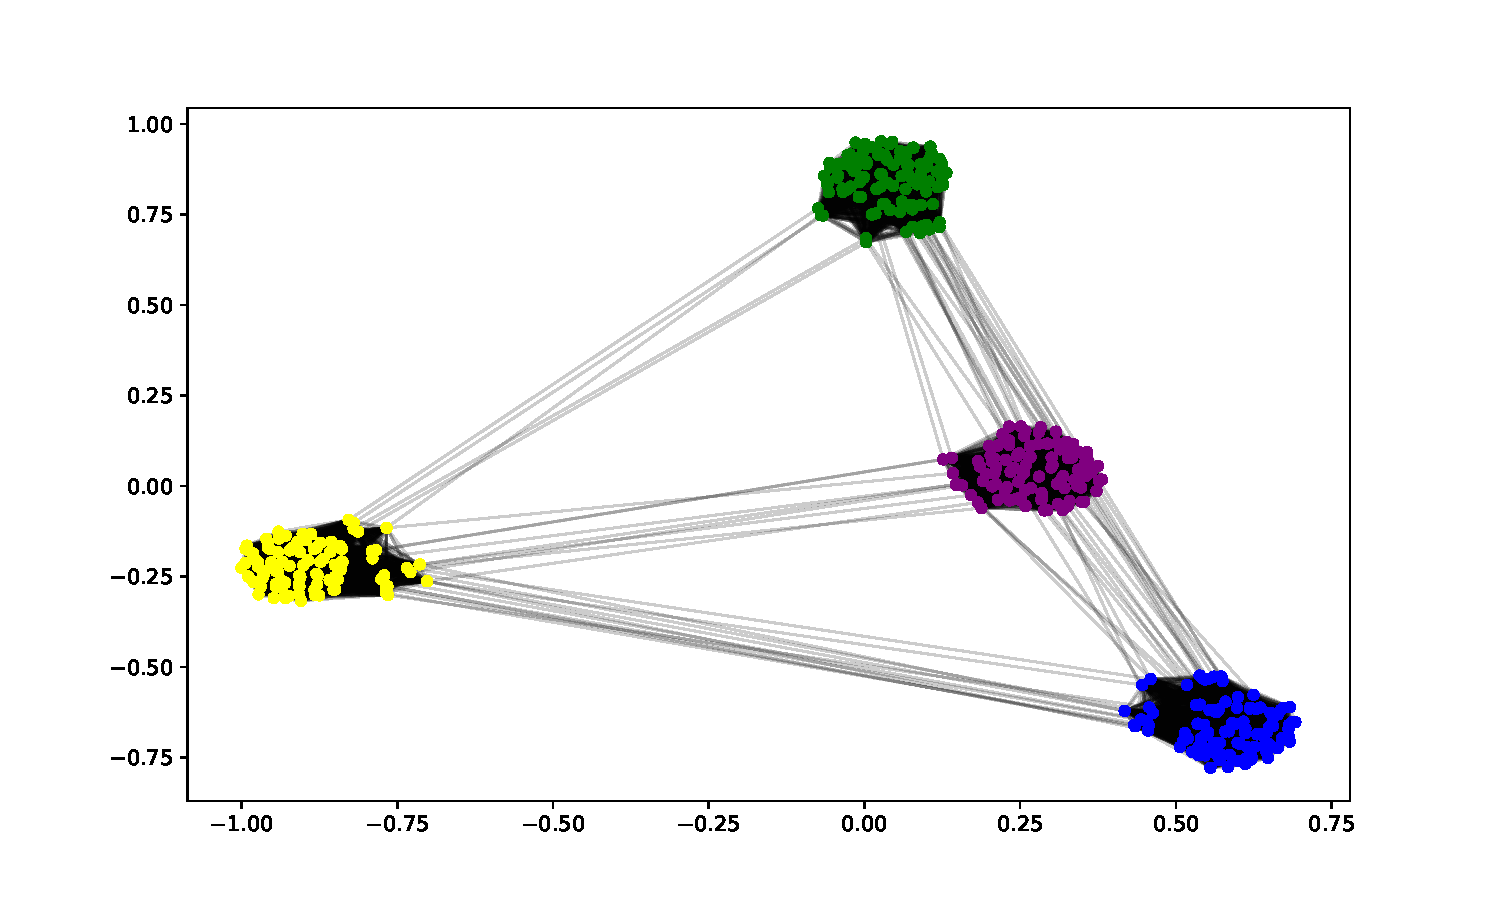
\includegraphics[width=\linewidth]{plots/images1/Louvain.pdf}
    \caption{Louvain algorithm}
    \label{fig:louv}
\end{figure}

It took $\approx 0.026$ seconds, it needs more time than the first two
methods, this is general to bigger graphs.

Let's compare the three methods :

On the amazon graph, Louvain needed \textbf{309 seconds} and found \textbf{242
communities}, Label Propagation needed \textbf{24.45 seconds} and found
\textbf{15063 communities} (which is enormous) and minimal Degree needed
\textbf{17.84 seconds} and found \textbf{86876 communities} (which is even more
enormous).

This means that the label propagation algorithm and our algorithm
(minimalDegree) detect more communities than the Louvain algorithm, they get
stuck in local minima, a solution to overcome this may be to do the same as in
the louvain algorithm, which is to consider the graph for which the nodes are
the communities and apply again the two algorithms until a reasonable number
of communities is found.

An other solution is to use the $min\_degree$ idea, for each node we will set
its label to the label of its neighbour with the lowest degree among the
neighbour with degree at least $min\_degree$.

 This is enough proof of the superiority of the Louvain algorithm. But let's
 see some numbers.
 We will use the function performance of the quality module of Networkx%
 \footnote{\url{https://networkx.github.io/documentation/latest/reference/%
 algorithms/generated/networkx.algorithms.community.quality.performance.html}}
 which gives : The performance of a partition is the ratio of the number of
 intra-community edges plus inter-community non-edges with the total number of
 potential edges.

Let's go back to the random graphs generated above, here is the results
obtained in the following order. (label propagation - minimal degree - Louvain)
With size being the number of communities found by the algorithm and perf
the performance of the algorithm.

\begin{figure}[!ht]
\centering
\begin{minipage}{.33\textwidth}
  \centering
  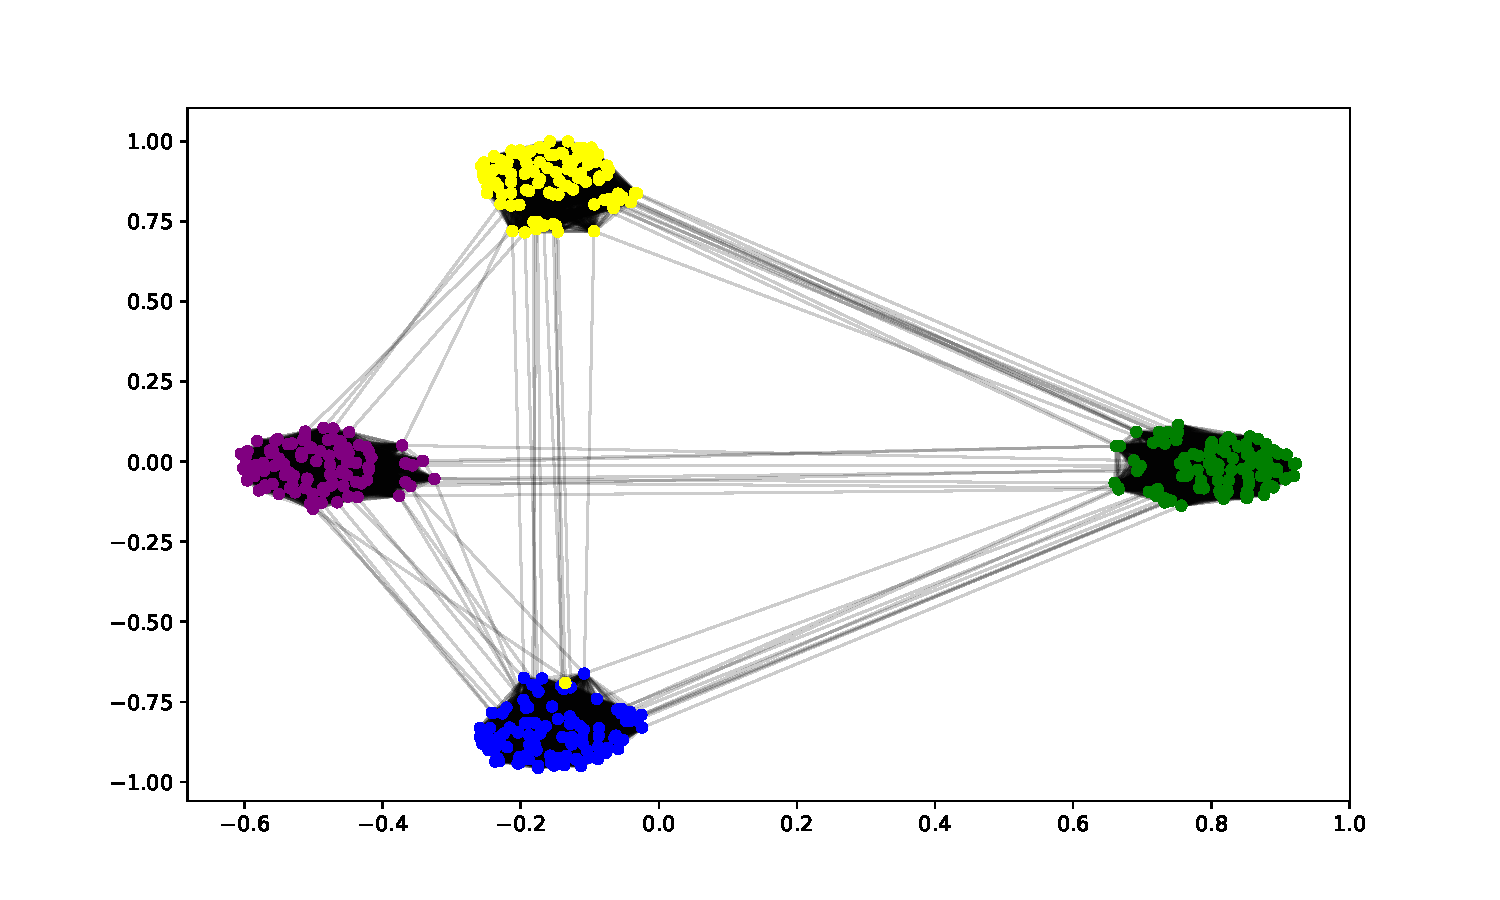
\includegraphics[width=\linewidth]{plots/images1/LabelPropagation.pdf}
  \caption*{size:4 perf:0.967}
\end{minipage}%
\begin{minipage}{.33\textwidth}
  \centering
  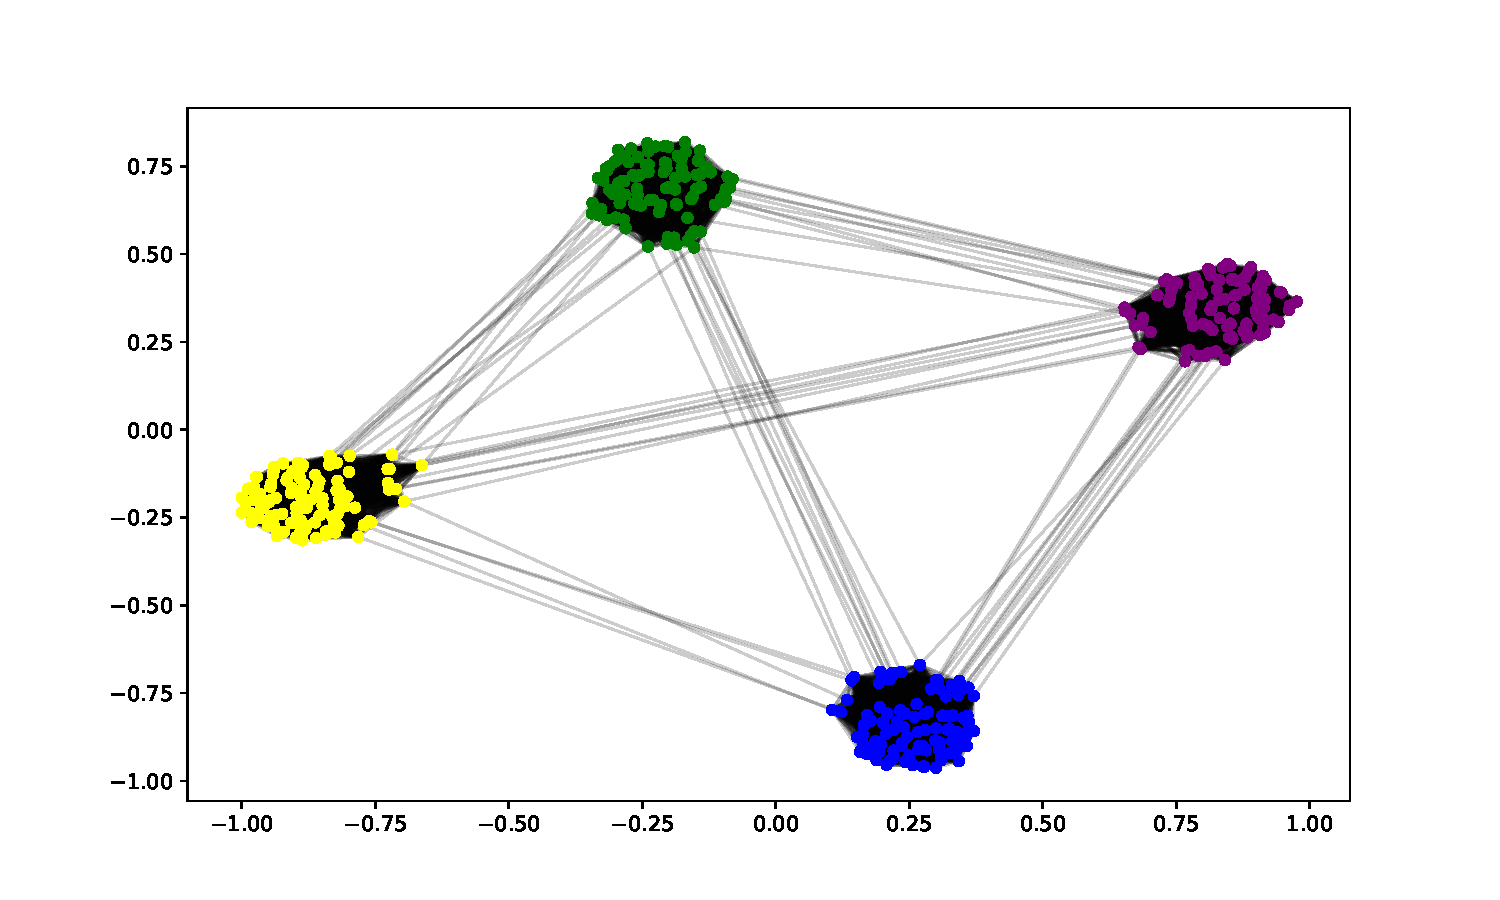
\includegraphics[width=\linewidth]{plots/images1/ex3minimalDegree.pdf}
  \caption*{size:4 perf:0.969}
\end{minipage}
\begin{minipage}{.33\textwidth}
  \centering
  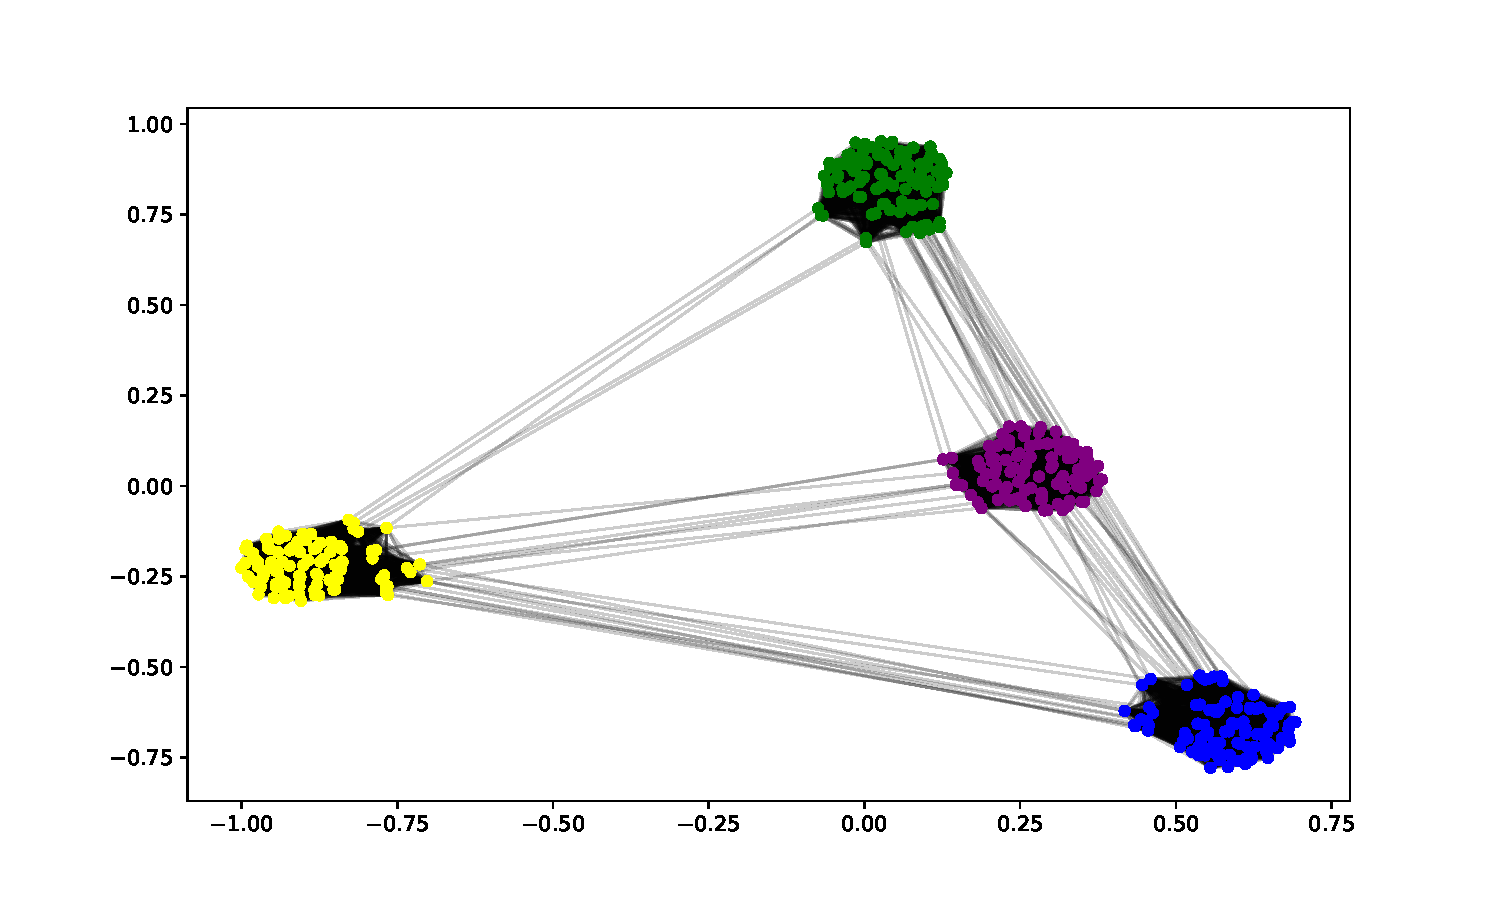
\includegraphics[width=\linewidth]{plots/images1/Louvain.pdf}
  \caption*{size:4 perf:0.969}
\end{minipage}
\caption{first graph}
\end{figure}



\begin{figure}[!ht]
\centering
\begin{minipage}{.33\textwidth}
  \centering
  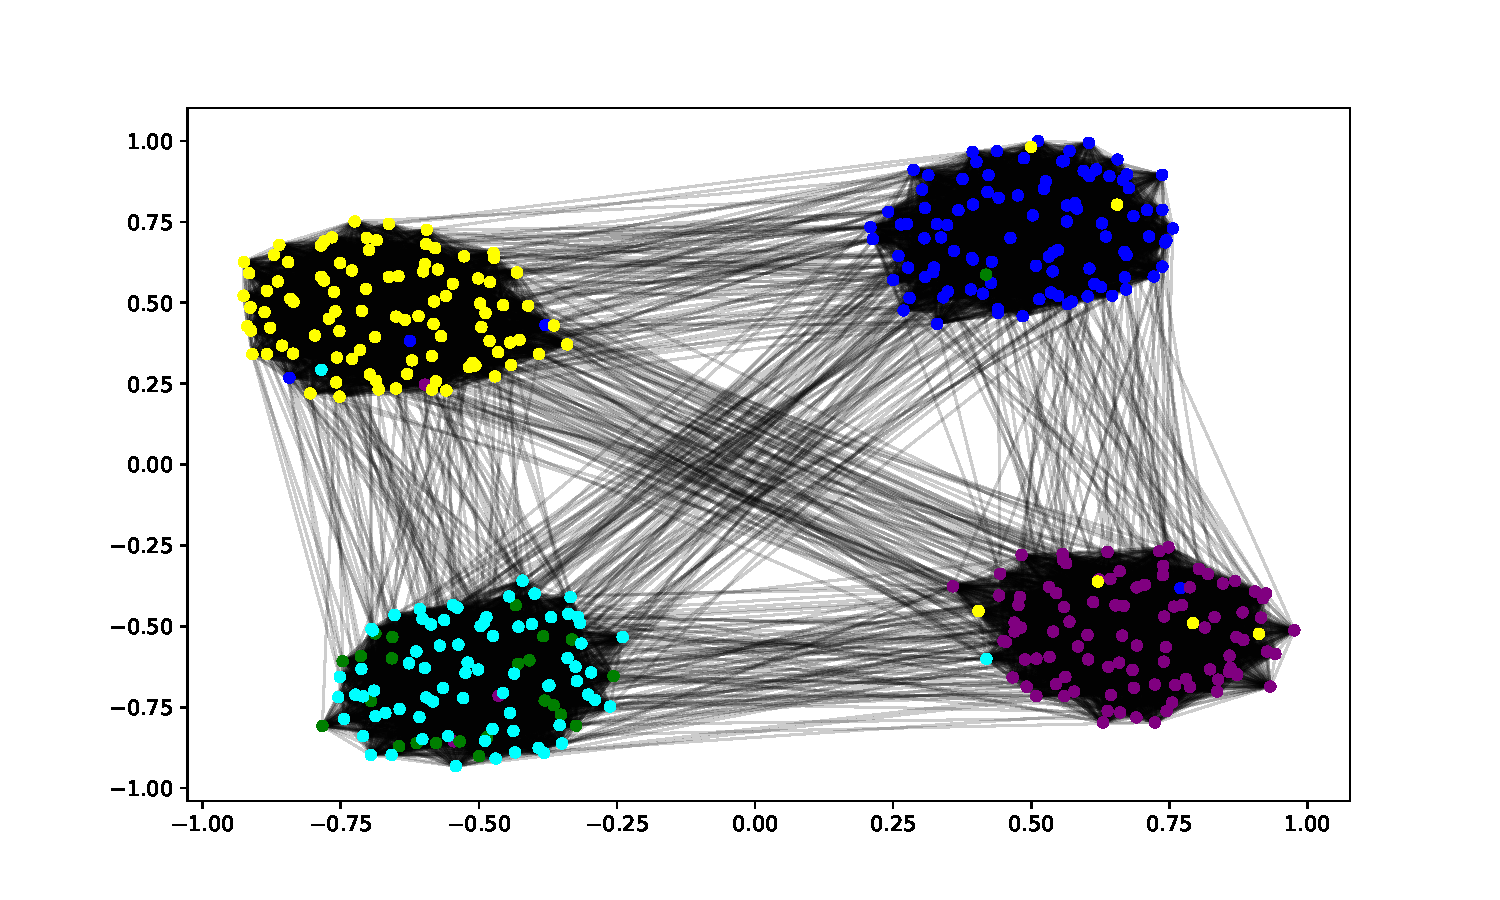
\includegraphics[width=\linewidth]{plots/images2/LabelPropagation.pdf}
  \caption*{size:5 perf:0.921}
\end{minipage}%
\begin{minipage}{.33\textwidth}
  \centering
  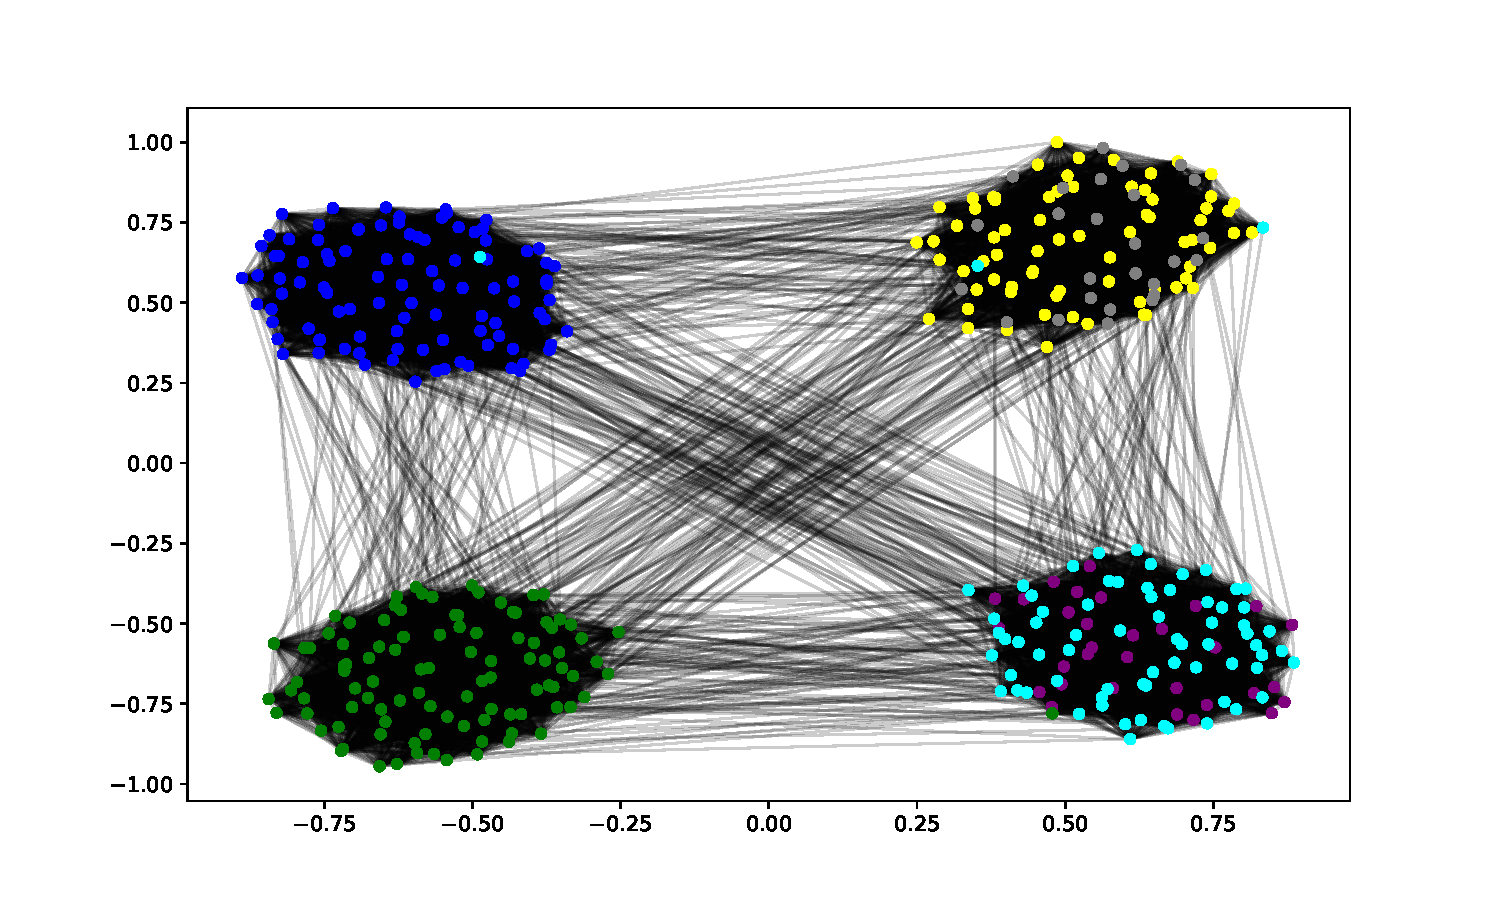
\includegraphics[width=\linewidth]{plots/images2/ex3minimalDegree.pdf}
  \caption*{size:6 perf:0.924 }
\end{minipage}
\begin{minipage}{.33\textwidth}
  \centering
  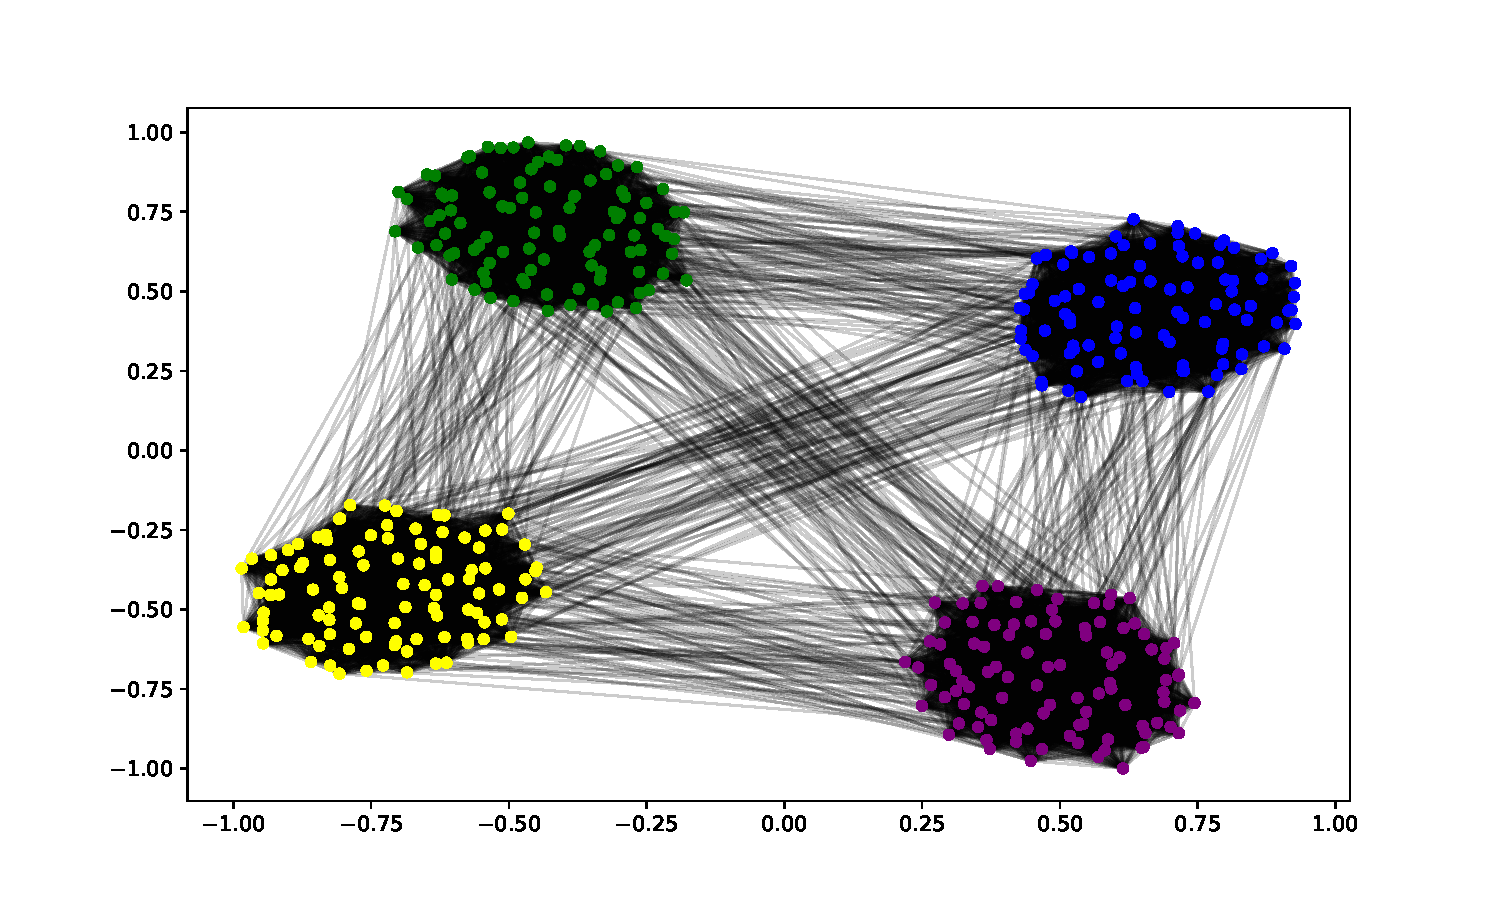
\includegraphics[width=\linewidth]{plots/images2/Louvain.pdf}
  \caption*{size: 4 perf: 0.970}
\end{minipage}
\caption{second graph}
\end{figure}


\begin{figure}[!ht]
\centering
\begin{minipage}{.33\textwidth}
  \centering
  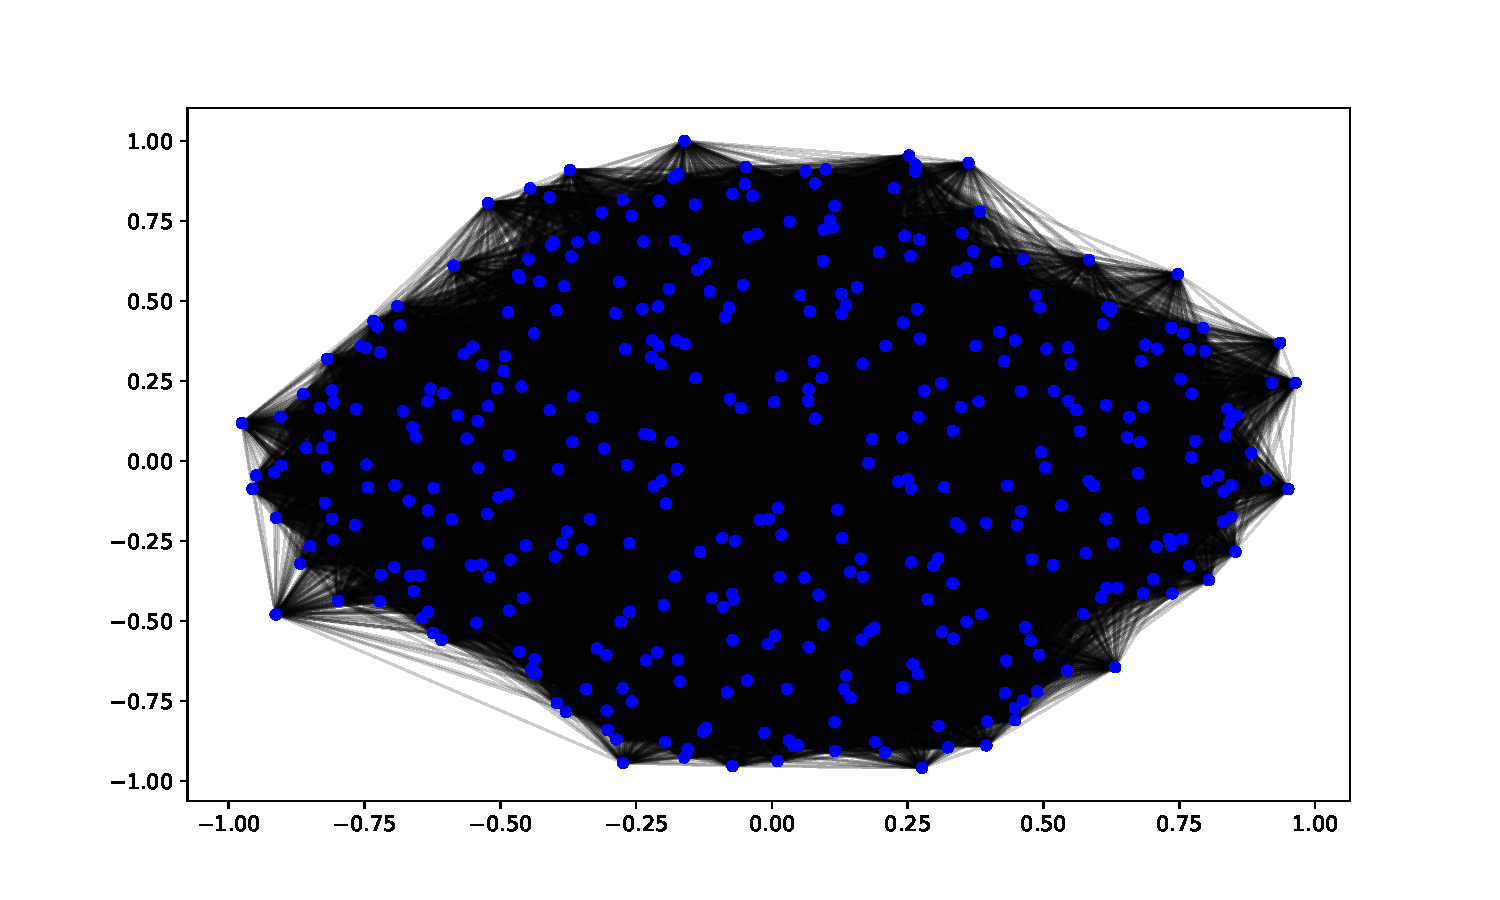
\includegraphics[width=\linewidth]{plots/images3/LabelPropagation.pdf}
  \caption*{size:1 perf:0.22}
\end{minipage}%
\begin{minipage}{.33\textwidth}
  \centering
  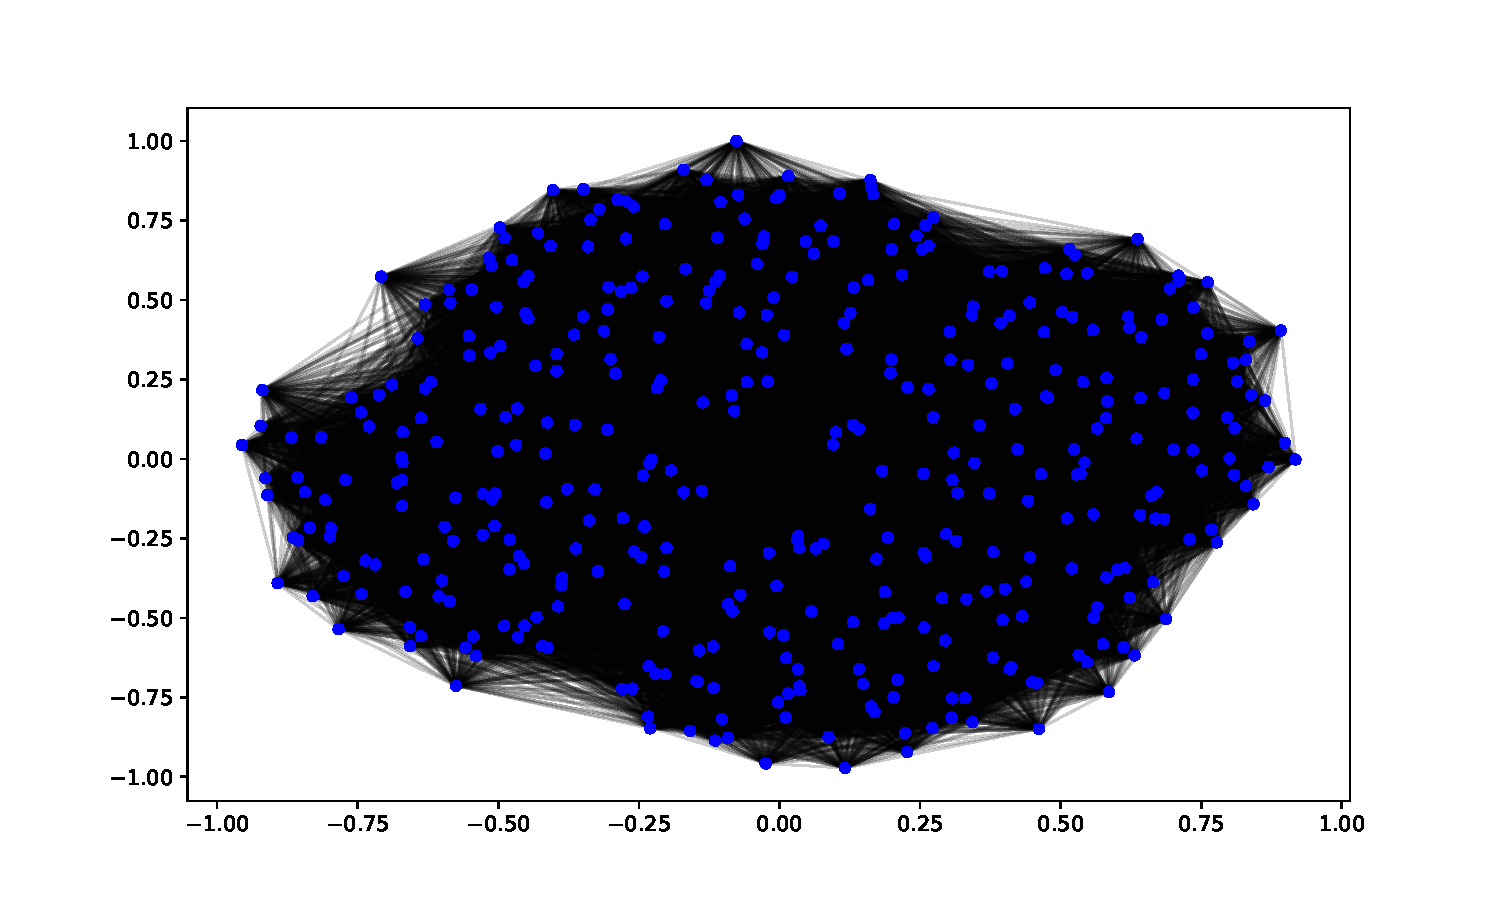
\includegraphics[width=\linewidth]{plots/images3/ex3minimalDegree.pdf}
  \caption*{size:1 perf:0.22}
\end{minipage}
\begin{minipage}{.33\textwidth}
  \centering
  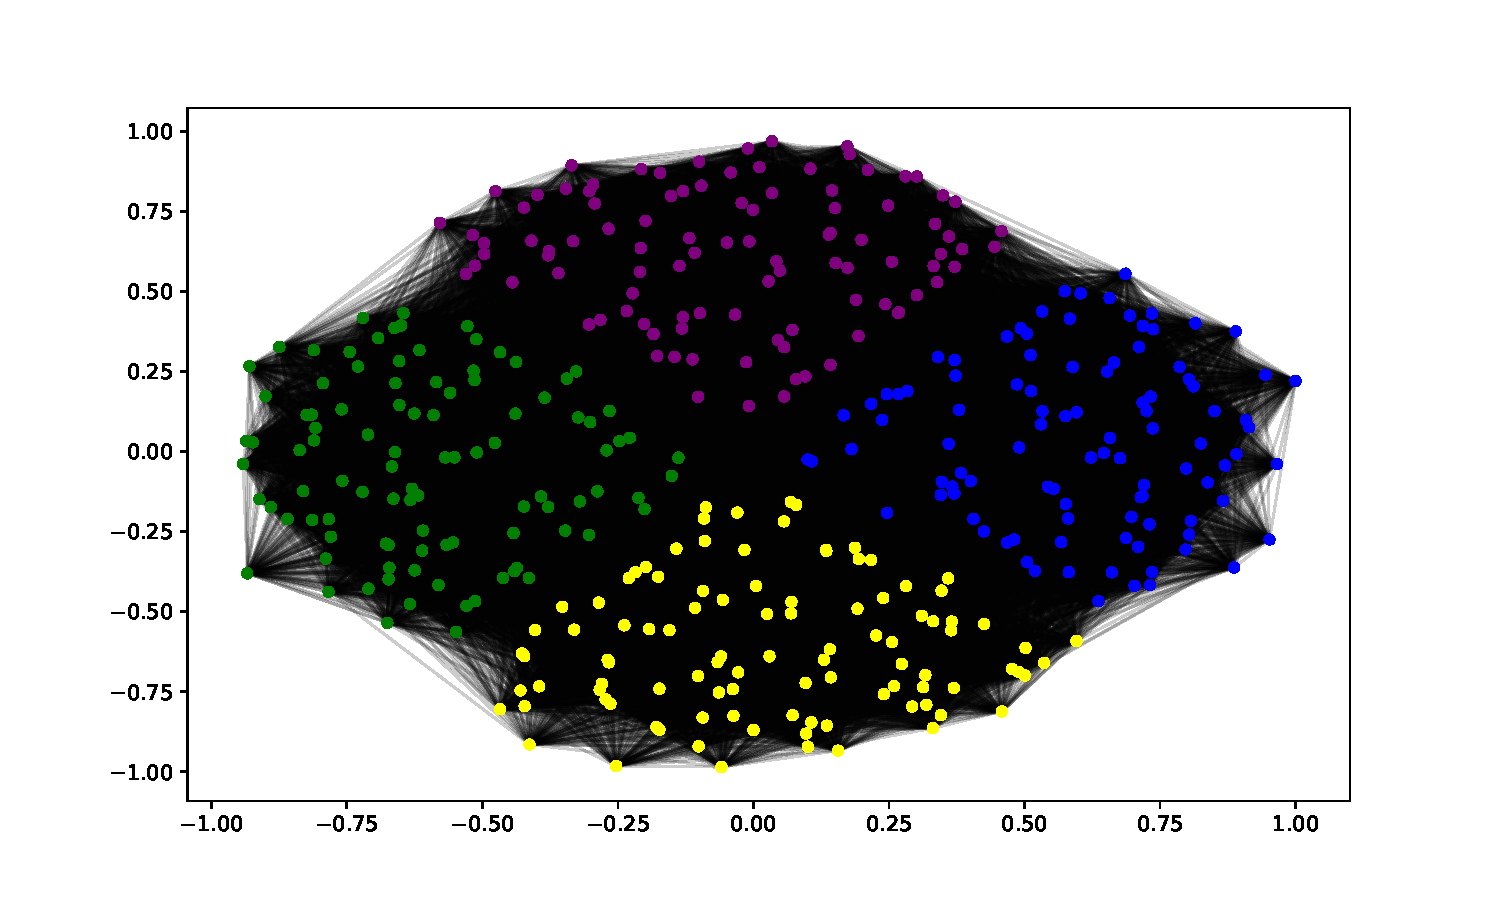
\includegraphics[width=\linewidth]{plots/images3/Louvain.pdf}
  \caption*{size:4 perf:0.970}
\end{minipage}
\caption{third graph}
\end{figure}
\newpage
All in all, Louvain is more robust than the other two algorithms, it can detect
the community structure very well even for graphs that are not very well
"separated" like the third graph.

By taking the $min\_degree$ parameter to be $\approx qN = 80$ we did better
with the minimal degree algorithm (performance $\approx$ 0.643), see figure
\ref{fig:9}.

\begin{figure}[!ht]
    \centering
    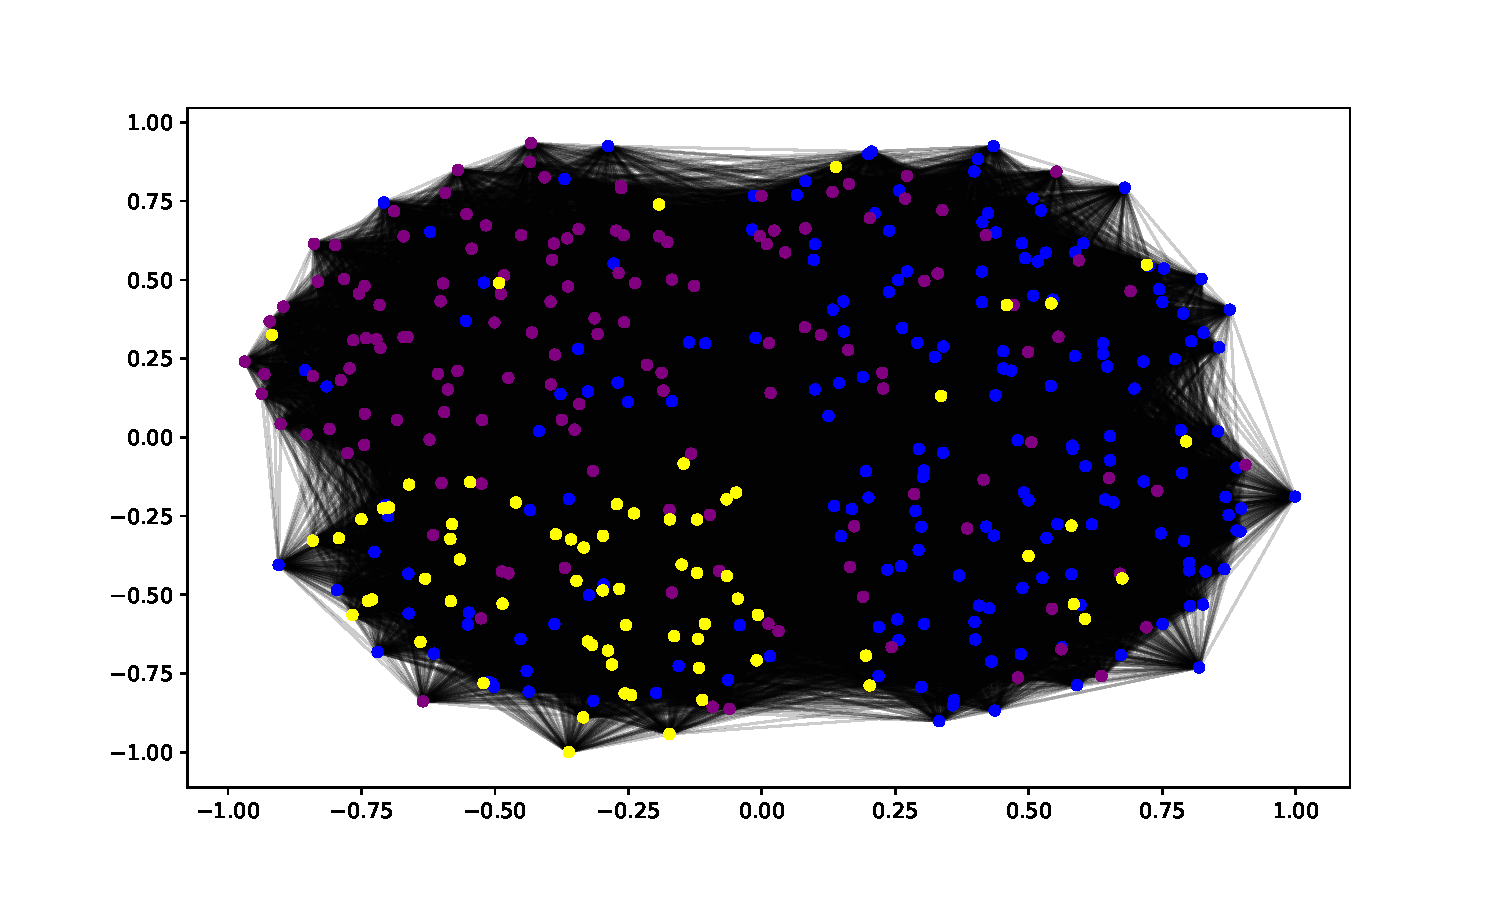
\includegraphics[width=\linewidth]{plots/ex3minimalDegree.pdf}
    \caption{Minimal degree with min\_degree=80}
    \label{fig:9}
\end{figure}
This shows that using this parameter we can actually hope to get out of bad
local optima.

\end{document}
